\subsection{Experimento II}\label{ch:experimento1}
El segundo experimento se trata de una prueba de apoyo a la investigación, que pone de manifiesto algunas limitaciones del robotario. El objetivo es obtener datos experimentales para validar un algoritmo que estima la posición relativa de un robot en movimiento respecto a otros, empleando medidas locales tomadas desde los robots sin necesidad de posicionamiento global. Este algoritmo está en fase de desarrollo\cite{hector}.\\
Dado un conjunto de robots en movimiento distribuidos en el plano, se puede considerar que en cada instante de tiempo los robots ocupan la posición de los vértices de un polígono. El algoritmo necesita conocer la variación de los ángulos internos del polígono así como la velocidad relativa de los robots para que cada uno determine la posición relativa de sus compañeros.
\subsection{Preparación del experimento}

\begin{figure}[!h]
	\centering
	\includegraphics[width=0.85\linewidth]{Demostracion/algoritmoExp2}
	\caption{Algoritmo de control del experimento 2}
	\label{fig:algexp2}
\end{figure}
\begin{figure}[!h]
	\centering
	\includegraphics[width=0.5\linewidth]{Demostracion/trianguloRobotsInicio}
	\caption{Posición inicial de los robots}
	\label{fig:isosceles}
\end{figure}
Inicialmente se planteó un escenario simplificado: Se emplean tres robots (R1,R2,R3) colocados de modo que sus posiciones iniciales formen un triángulo isósceles tal y como se muestra en la Figura~\ref{fig:isosceles}. Cada robot lleva un identificador en su parte frontal, de modo que su posición relativa puede ser estimada por sus compañeros mediante las cámaras que llevan a bordo empleando para ello las funciones proporcionadas por OpenCV. Que se comentó en el capitulo~\ref{ch:localizacionRobots}.\\
Los robots R1 y R3 permanecen en reposo todo el tiempo. El robot R2, ocupa el vértice de los dos lados iguales del triángulo, y se mueve a lo largo de su bisectriz. Mientras se desplaza, emplea la cámara de abordo para detectar la posición relativa de los robots R1 y R3, mediante los identificadores que llevan colocados.\\
Las posiciones relativas obtenidas se emplean en primer lugar como referencia para comparar con los resultados del algoritmo. Además, a partir de ellas, se estima el ángulo $\alpha_{1,2,3}$, que es el ángulo que ve el robot2 con la dirección desde el robot1 hasta el robot3. A partir de este ángulo se obtienen los otros dos. Por último, para completar los datos necesarios para validar el algoritmo, se estima la velocidad del robot2 empleando las lecturas de sus encoders y se guardan en un fichero que almacena la raspberryPi.\\
Para adquirir el numero suficiente de datos se hace que el robot en movimiento avance y retroceda a lo largo de la bisectriz del triángulo. Además se crea una ley de control que se detalla en la Figura~\ref{fig:algexp2} para que el robot siga la bisectriz mientras avanza y retrocede.\\
En este experimento el control, el registro de las posiciones relativas de donde se sacan los ángulos y las velocidades se hace desde la raspberryPi. La comunicación entre la placa de Arduino y la raspberryPi se realiza mediante puerto serie.Como se indicó en la sección~\ref{ch:controlador} los motores de las ruedas de los robots no son iguales. Esto hace que ya en el arranque el robot R2 se separe de la bisectriz. Aunque el algoritmo de control, devuelve el robot a su ruta. \\
\begin{figure}[!ht]
	\centering
	\includegraphics[width=0.65\linewidth]{Demostracion/trayectoriaExp2}
	\caption{Trayectoria del robot 2}
	\label{fig:trayectoriaExp2}
\end{figure}
En la Figura~\ref{fig:trayectoriaExp2} se tiene las posiciones registradas durante el experimento. Se puede apreciar como el robot intenta mantenerse en la bisectriz a pesar de las desviaciones que sufre el robot. Debido a que la dimensión del robotario es pequeña, no recorre la suficiente distancia para que la corrección sea efectiva y justo cuando está corrigiendo el robot cambia de sentido de avance. Por otro lado, las pequeñas paradas del robot para reorientarse en busca de la bisectriz, hacen que parte de los datos no sean válidos para el algoritmo, que necesita una variación de ángulos suave.\\
Para poder obtener datos válidos se modificó el experimento, haciendo que el robot1 obtuviera las posiciones relativas de los demás robots con su cámara de a bordo. De este modo es posible determinar los tres ángulos sin necesidad de que el triángulo formado por los tres robots sea isósceles en todo momento. Además se decidió emplear control manual del robot para tratar de hacer más suave el control de rumbo.\\

\subsection{Resultados}
La descripción del algoritmo desarrollado\cite{hector} queda fuera del alcance de este trabajo. En las Figuras~\ref{fig:teorema1}~\ref{fig:teorema2} se muestran una gráficas, cortesía de los autores del algoritmo, donde se compara la posición medidas por el robot2, mediante los Markers con la que se obtiene mediante su algoritmo, aplicando dos métodos distintos. En el segundo caso se hace uso de un estimador, los resultados son bastante aceptables, teniendo en cuenta las limitaciones del robotario

\begin{figure}[!h]
	\begin{subfigure}[b]{0.55\linewidth}
		\centering
		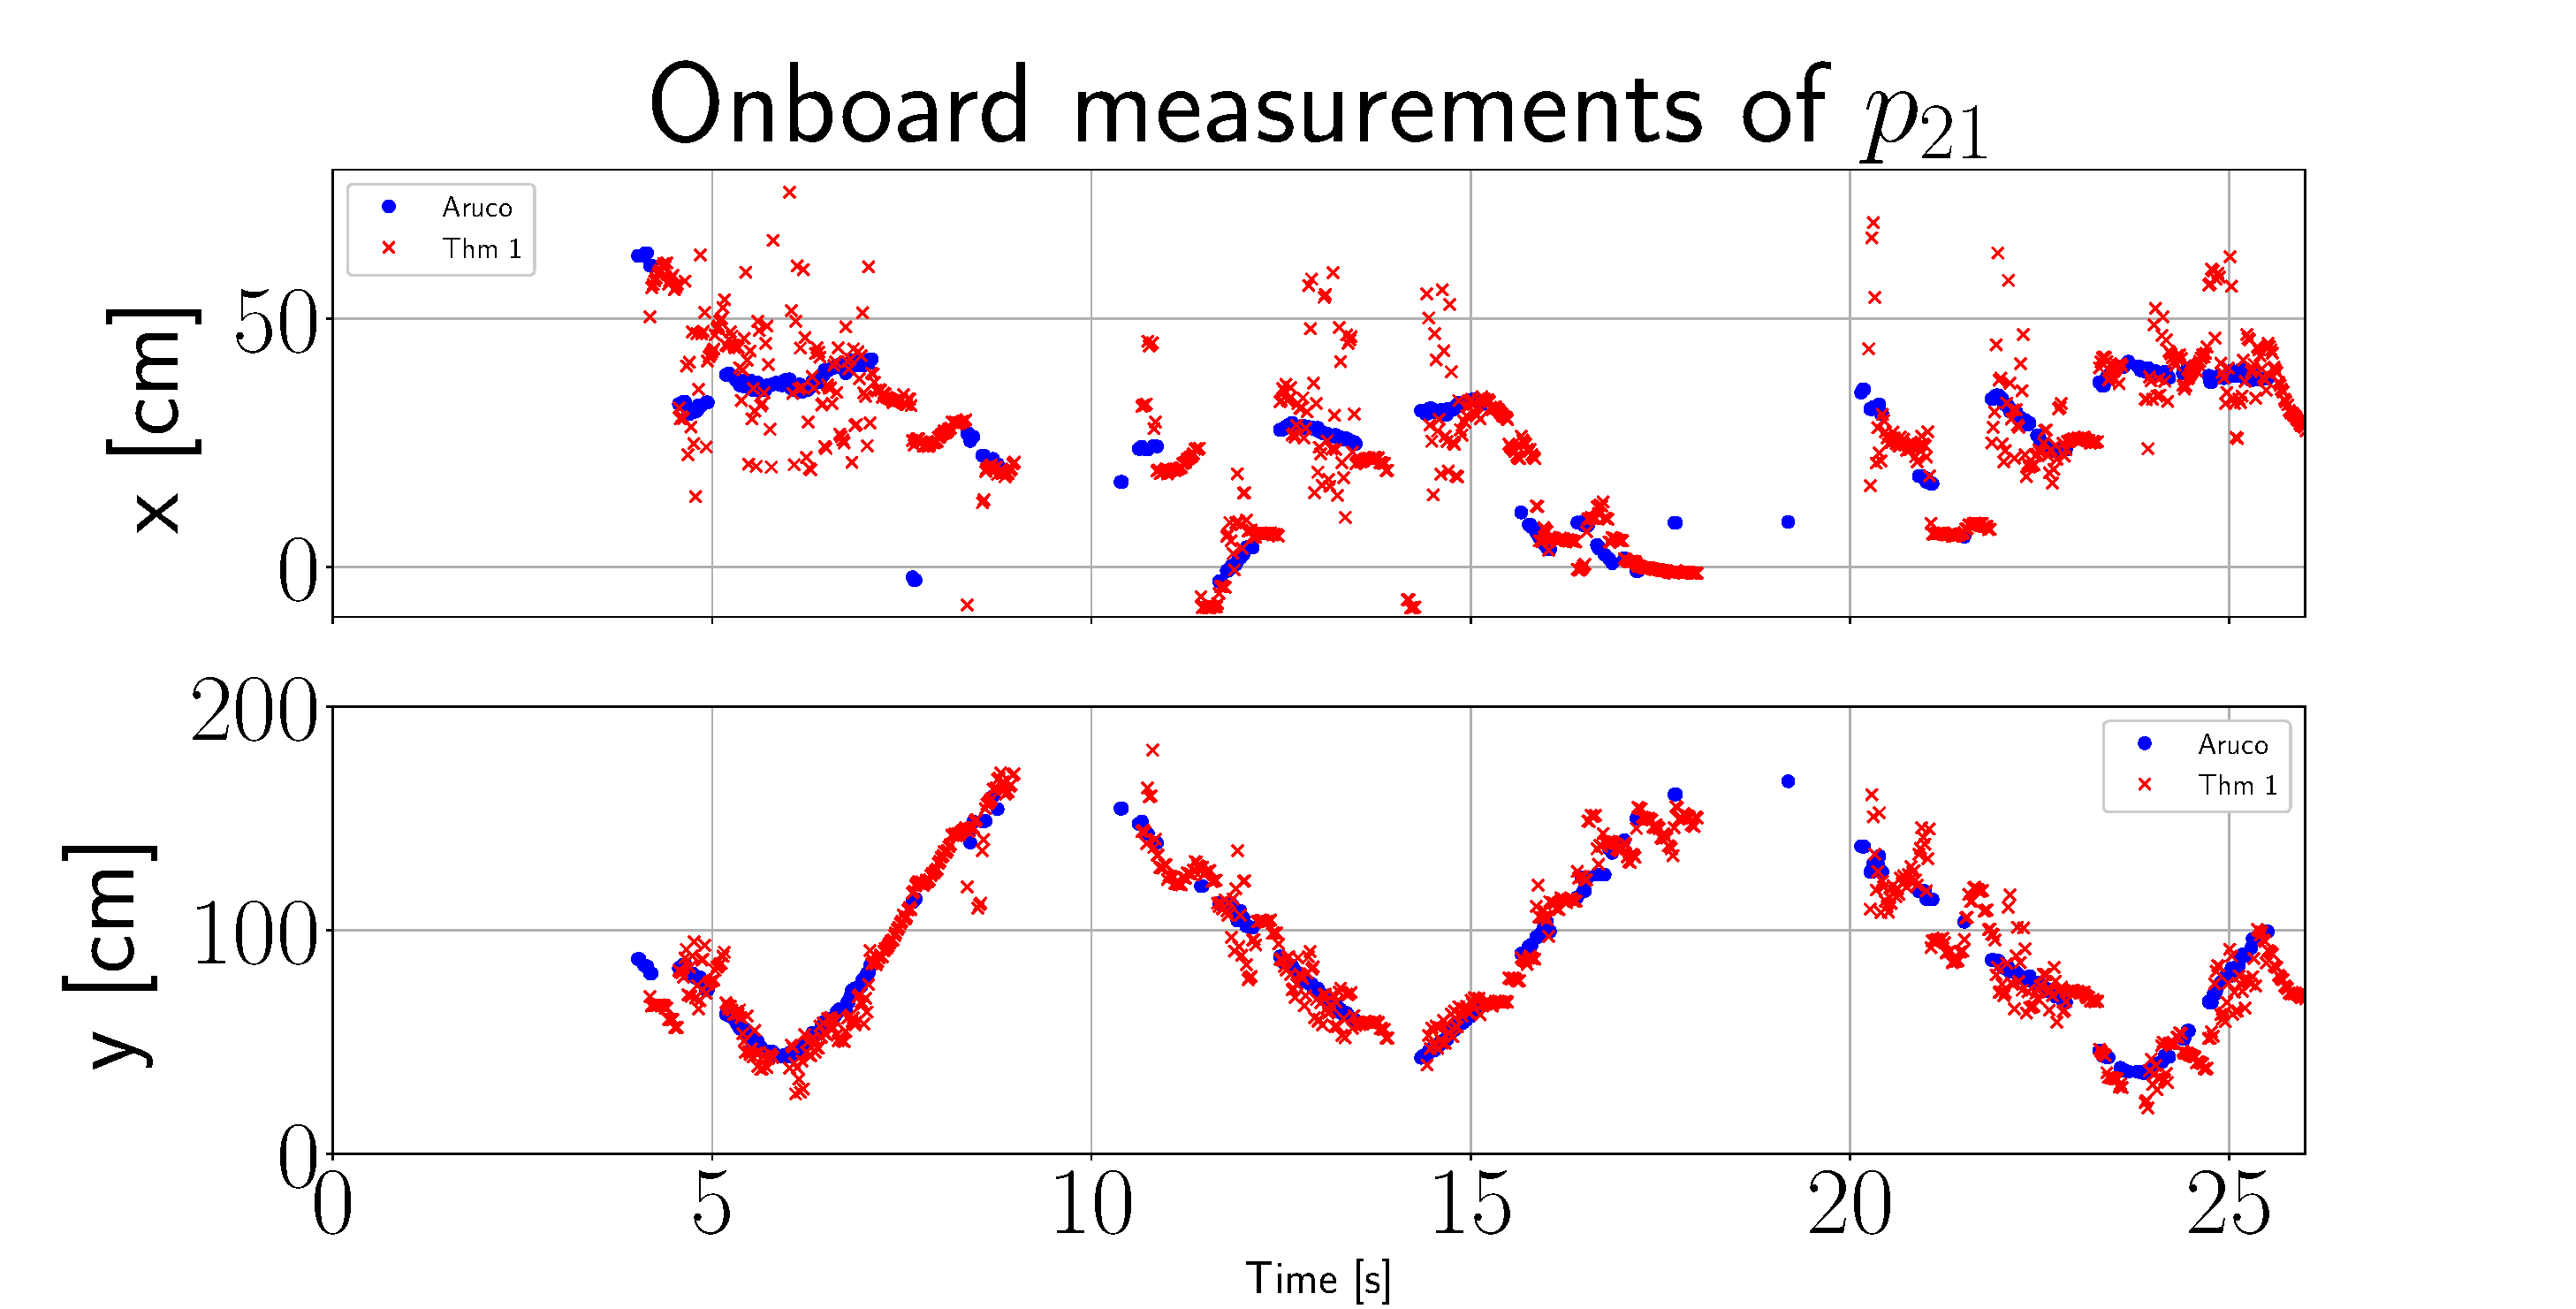
\includegraphics[width=0.7\linewidth]{Demostracion/p21_thm1}
		\caption{Posición relativa robot2-robot1}
		\label{fig:thm1r21}
	\end{subfigure}
	\quad
	\begin{subfigure}[b]{0.55\linewidth}
		\centering
		\includegraphics[width=0.7\linewidth]{Demostracion/p23_thm1}
		\caption{Posición relativa robot2-robot3}
		\label{fig:thm1r23}
	\end{subfigure}
	\caption{Resultados aplicando el método 1}
	\label{fig:teorema1}
\end{figure}
\begin{figure}[!h]
	\begin{subfigure}[b]{0.55\linewidth}
		\centering
		\includegraphics[width=0.7\linewidth]{Demostracion/p21_thm2}
		\caption{Posición relativa robot2-robot1}
		\label{fig:thm2r21}
	\end{subfigure}
	\quad
	\begin{subfigure}[b]{0.55\linewidth}
		\centering
		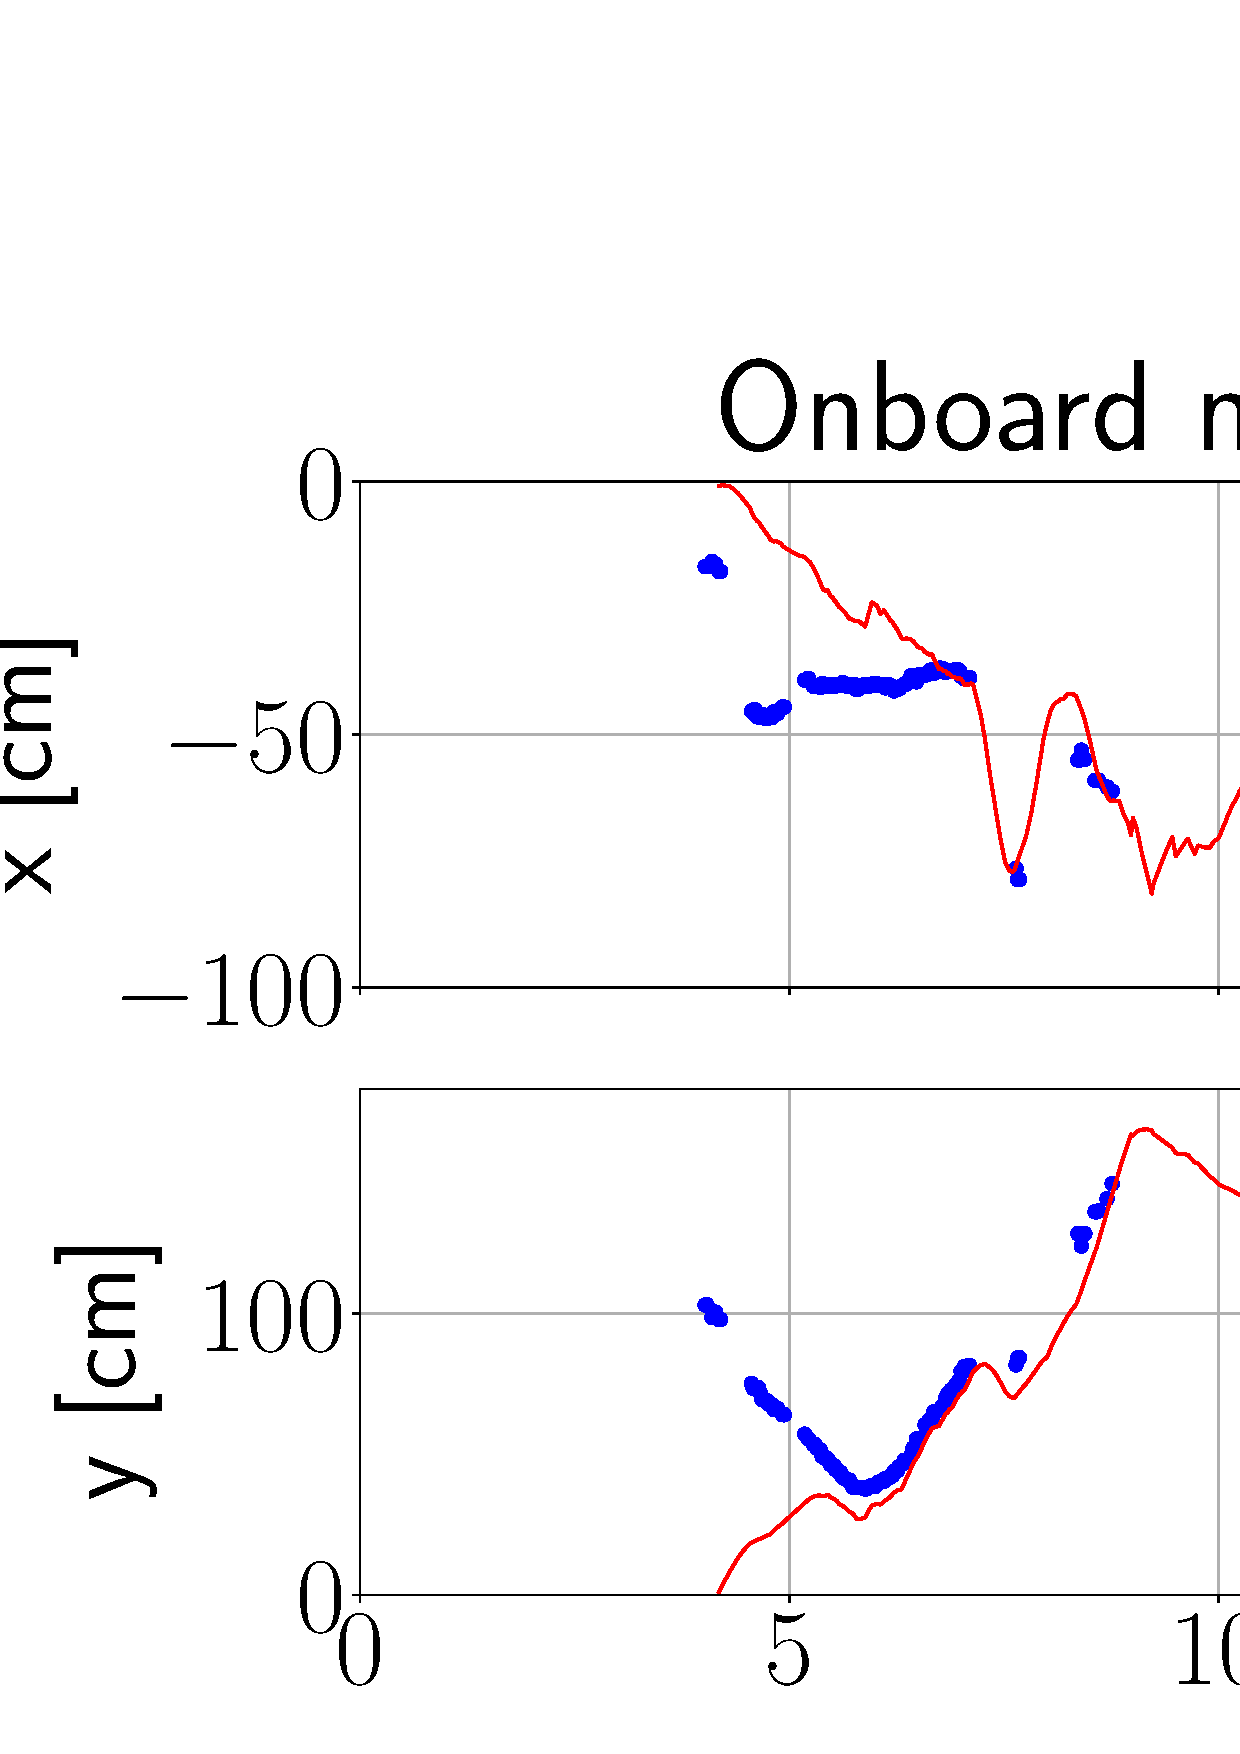
\includegraphics[width=0.7\linewidth]{Demostracion/p23_thm2}
		\caption{Posición relativa robot2-robot3}
		\label{fig:thm2r23}
	\end{subfigure}
	\caption{Resultados aplicando el método 2(estimador)}
	\label{fig:teorema2}
\end{figure}
Los puntos azules son el resultado del algoritmo y en rojo se tiene la medición realizada por el robot2.

\newpage


